%%%%%%%%%%%%%%%%%%%%%%%%%%%%%%%%%%%%%%%%%
% Beamer Presentation
% Standard LaTeX Template used for creating presentation of Firebird-V Robot and other tutorials. 
% Author: Saurav Shandilya (e-Yantra Team)
% Reference: www.LaTeXTemplates.com Version 1.0 (10/11/12)
%
%%%%%%%%%%%%%%%%%%%%%%%%%%%%%%%%%%%%%%%%%

%----------------------------------------------------------------------------------------
%	PACKAGES AND THEMES
%----------------------------------------------------------------------------------------
		
\documentclass[table,10pt,red]{beamer}	% First line -- Define document class as Beamer which is used for creating presentation using Latex
\setbeamercolor{alerted text}{fg=blue} 	% Sets color of highlighted text during presentation.  
 

% The Beamer class comes with a number of default slide themes
% which change the colors and layouts of slides. Below this is a list
% of all the themes, uncomment each in turn to see what they look like.

%\usetheme{default}
%\usetheme{AnnArbor}
%\usetheme{Antibes}
%\usetheme{Bergen}
%\usetheme{Berkeley}
\usetheme{Berlin}		%used theme in present documents.
%\usetheme{Boadilla}
%\usetheme{CambridgeUS}
%\usetheme{Copenhagen}
%\usetheme{Darmstadt}
%\usetheme{Dresden}
%\usetheme{Frankfurt}
%\usetheme{Goettingen}
%\usetheme{Hannover}
%\usetheme{Ilmenau}
%\usetheme{JuanLesPins}
%\usetheme{Luebeck}
%\usetheme{Madrid}
%\usetheme{Malmoe}
%\usetheme{Marburg}
%\usetheme{Montpellier}
%\usetheme{PaloAlto}
%\usetheme{Pittsburgh}
%\usetheme{Rochester}
%\usetheme{Singapore}
%\usetheme{Szeged}
%\usetheme{Warsaw}

% As well as themes, the Beamer class has a number of color themes
% for any slide theme. Uncomment each of these in turn to see how it
% changes the colors of your current slide theme.

%\usecolortheme{albatross}
%\usecolortheme{beaver}
%\usecolortheme{beetle}
%\usecolortheme{crane}
%\usecolortheme{dolphin}
%\usecolortheme{dove}
%\usecolortheme{fly}
%\usecolortheme{lily}
%\usecolortheme{orchid}
%\usecolortheme{rose}
%\usecolortheme{seagull}
%\usecolortheme{seahorse}
%\usecolortheme{whale}
%\usecolortheme{wolverine}

%\setbeamertemplate{footline} % To remove the footer line in all slides uncomment this line
%\setbeamertemplate{footline}[page number] % To replace the footer line in all slides with a simple slide count uncomment this line

%\setbeamertemplate{navigation symbols}{} % To remove the navigation symbols from the bottom of all slides uncomment this line
%}

%------------------------------------------------------------------------------------------
%	\usepackage is required for including various features like images, table, references etc.
%	Packages must be installed before using. These can be istalled through package manager. 
%   Various packages have dependencies and for using such packages all dependent packages must be used. 
%-----------------------------------------------------------------------------------------
\usepackage{beamerthemeshadow} % theme shadow for visual 
\usepackage{beamerthemesplit} % Creates minipage (for showing multiple images and text) on same page  
\usepackage{graphicx} % Allows including images
\usepackage{booktabs} % Allows the use of \toprule, \midrule and \bottomrule in tables
\usepackage{xcolor}
\usepackage{booktabs,array}
\usepackage{listings}
\usepackage{hyperref}	% Required for including hyperlink in document
\usepackage{verbatim,moreverb} % Required for including code snippet.
\usepackage{colortbl}
\usepackage{multirow}	% Required for creating multiple row tables
\usepackage{tikz}		% Required for drawing shapes such as circles, arrowed line, etc. 
\usetikzlibrary{arrows}

% logo
\logo{
\includegraphics[height=1cm]{iitblogo.pdf}} % includes logo at bottom of all slides 
\definecolor{comment}{HTML}{22ab22}
\addtobeamertemplate{block begin}{%
  \setlength{\textwidth}{0.9\textwidth}%
}{}

\addtobeamertemplate{block alerted begin}{%
  \setlength{\textwidth}{0.9\textwidth}%
}{}

\addtobeamertemplate{block example begin}{%
  \setlength{\textwidth}{0.9\textwidth}%
}{}
%----------------------------------------------------------------------------------------
%	TITLE PAGE
%----------------------------------------------------------------------------------------
% sf family, bold font
\sffamily \bfseries
% content inside [] appears at bottom of all page. content inside {} appears on first page as title. double backslash means line change 
\title
[
	Firebird LPC2148 ARM7 Robotics Research Platform	% bottom of all page
	\hspace{0.5cm}
	\insertframenumber/\inserttotalframenumber
]
{
	Stepper Motor Interfacing with Firebird V LPC2148 ARM7
}

\author
[
	www.e-yantra.org 	%Name at bottom of all page 
]
% author name on title slide
{
  Joel M. Pinto and Vishal Rajai\\
  eYantra Summer Internship -- 2014\\
  Embedded Real-Time Systems Lab\\
  Indian Institute of Technology, Bombay\\
}
\date
{
IIT Bombay \\ {\today}	%\today picks system date on title slide
}

\begin{document}

\begin{frame}
	\titlepage
	%Hello everyone! Welcome to the video tutorial on Firebird V robotics research platform. This platform is based on the LPC2148 microcontroller from the ARM7 family. In this tutorial we will learn about stepper motors, ways to control them and how to interface a stepper motor with the Firebird V robot.
\end{frame}

\begin{frame}
	\frametitle{Agenda for Discussion}
	
	\tableofcontents
	%Let's see the agenda for discusion in this tutorial.
	%First we will have an introduction where we will discuss what is a stepper motor and its types.
	%Then we will move on to learn how to control a stepper motor in different stepping sequences like wave, full and half stepping modes followed by a comparison of the three stepping modes.
	%Then we will have a short demonstration of how to identify the wires of a usually unlabelled stepper motor.
	%This will be followed by a discussion of the circuitry required to drive a stepper motor and then finally we will jump on to actually programming the robot to control the stepper motor.
\end{frame}

\section{Introduction}
\subsection{What is a stepper motor?}
\begin{frame}
	\frametitle{What is a stepper motor?}
		\begin{minipage}[c]{0.6\textwidth}
			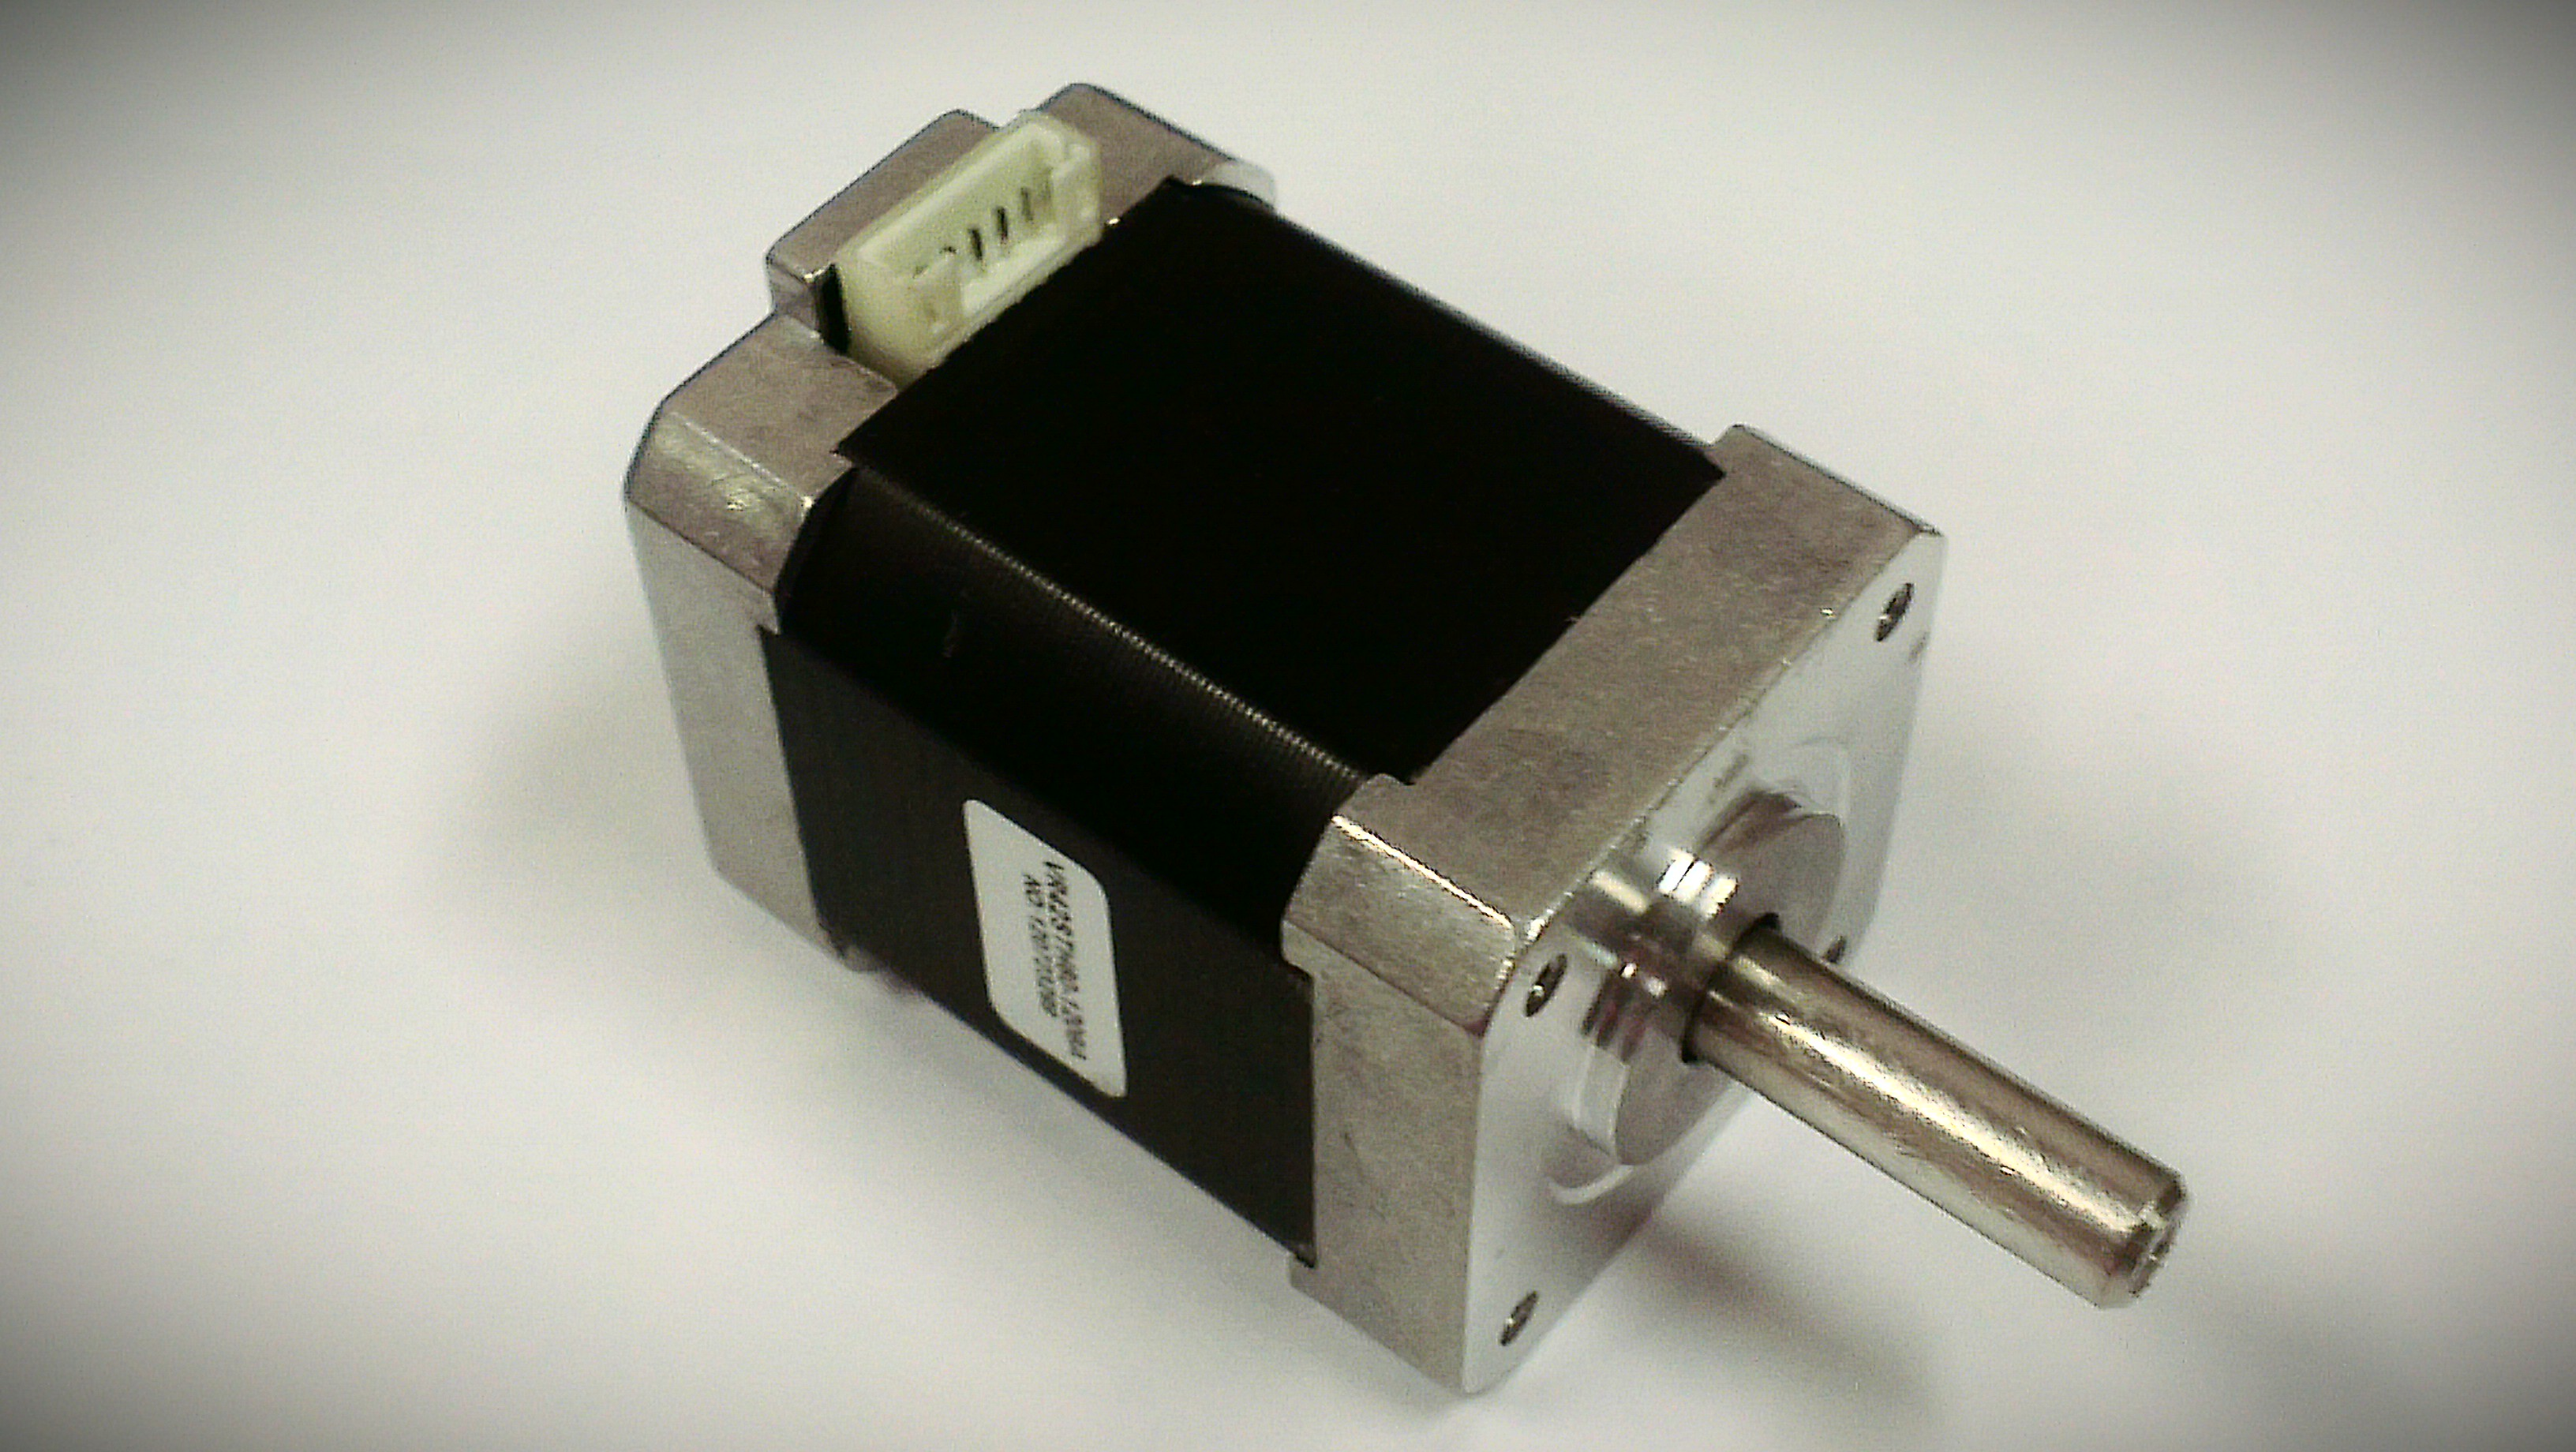
\includegraphics[width=\linewidth]{IMAG0758_1}
		\end{minipage}
	\pause
	%So the first question that arises is, What is a stepper motor? A stepper motor is a special kind of motor,
	\hfill
		\begin{minipage}[c]{0.3\textwidth}
			\begin{enumerate}
				\item <+-|alert@+> Rotates in discrete steps
				%whose rotation is divided into dicrete steps which allow precise control over its angle.
				\item <+-|alert@+> Can hold or move to a position
				%It can be commanded to hold a step or move to the next step.
			\end{enumerate}
		\end{minipage}   
\end{frame}

\subsection{Types of Stepper Motors}
\begin{frame}
	\frametitle{Types of Stepper Motors}
	\pause
	%Types
	%Steppers are mainly classified on the basis of their internal wiring. These classes are as follows.
	\begin{minipage}[c]{0.45\textwidth}
	\begin{itemize}
		\item Bipolar
			\begin{itemize}
				\item Has 4 wires
				
			\end{itemize}
	\end{itemize}
	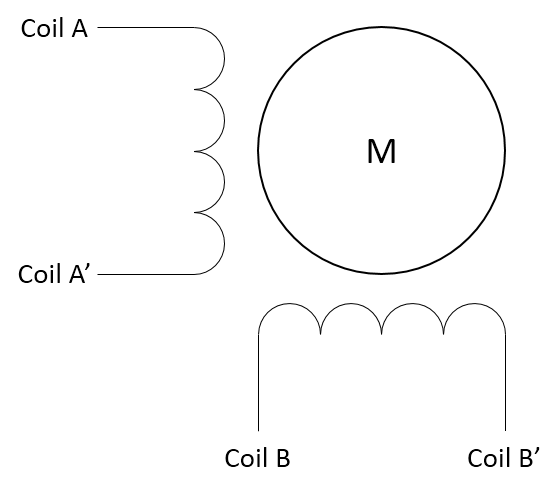
\includegraphics[width=\linewidth]{Bipolar}
	\end{minipage}
	\pause
	%Bipolar Steppers usually have 4 wires to control them and their drivers are complex		
	\begin{minipage}[c]{0.45\textwidth}
		\begin{itemize}
			\item Unipolar
				\begin{itemize}
					\item Has 5 or 6 wires
					
				\end{itemize}
		\end{itemize}
		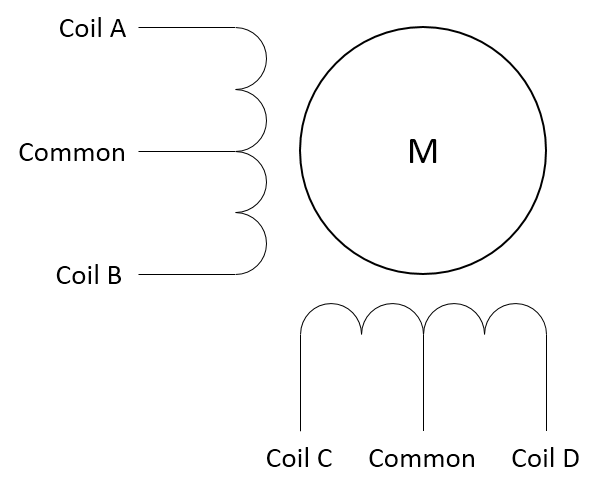
\includegraphics[width=\linewidth]{Unipolar}
	\end{minipage}
	\pause
	%Unipolar Steppers on the other hand have 5 or 6 wires and are relatively easier to drive
	
	We will use a unipolar stepper motor.
	%Since, Unipolar motors are commonly used, we will be using them in this tutorial
\end{frame}
\section{Controlling a Stepper Motor}

\subsection{Stepping sequences}

\begin{frame}
	\frametitle{Stepping sequences}
	\pause
	%Moving on to how to control a stepper motor, a stepper motor can be controlled by sending specific sequences of signals to its wires. The different stepping sequences are
	\begin{enumerate}
		\item <+-|alert@+> Wave Stepping
		%Wave Stepping
		\item <+-|alert@+> Full Stepping
		%Full Stepping
		\item <+-|alert@+> Half Stepping
		%and Half Stepping
	\end{enumerate}
	%We will now see and understand how to use each one of them.
\end{frame}

\subsection{Wave Stepping}

\begin{frame}
	\frametitle{Wave Stepping}
	\pause
	%Wave stepping
	%It involves exciting each coil turn by turn in a circular fashion.
	\begin{table}
		\begin{tabular}{c c c c c}
			\toprule
			\textbf{Step} & \textbf{Coil A} & \textbf{Coil B} & \textbf{Coil C} & \textbf{Coil D}\\
			\midrule
			1 & 1 & 0 & 0 & 0 \\
			2 & 0 & 1 & 0 & 0 \\
			3 & 0 & 0 & 1 & 0 \\
			4 & 0 & 0 & 0 & 1 \\
			\bottomrule
		\end{tabular}
		\caption{Wave stepping sequence}
	\end{table}
	%The table shows which coils are to be excited for generating the wave stepping sequence. Here a 1 denotes ON whereas a 0 denotes OFF. To rotate the stepper motor in one direction, we send the sequence, 1-2-3-4-1 and so on while for the opposite direction, we send the sequence in reverse, i.e., 4-3-2-1-4 and so on.
\end{frame}

\begin{frame}
	\frametitle{Wave Stepping (contd.)}
	%Shown here is an illustration that depicts the direction of the rotor inside a stepper motor in the wave stepping sequence. The rotor points to the excited coil at that instant. When coil A is excited, the rotor aligns itself to point to it. Next, when coil B is excited, the rotor turns to align itself again. This process repeats for the other coils.
	\begin{minipage}[c]{0.24\textwidth}
		\begin{figure}
			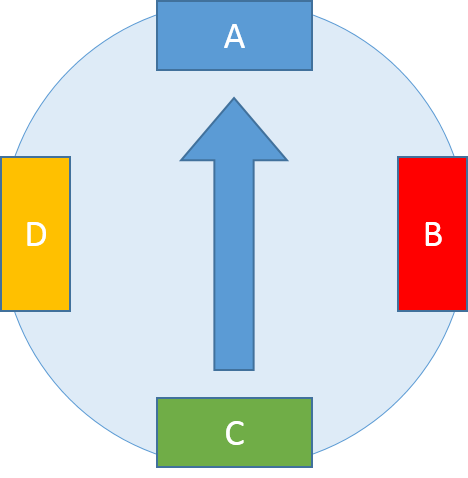
\includegraphics[width=0.9\linewidth]{step1}
		\end{figure}
	\end{minipage}
	\begin{minipage}[c]{0.24\textwidth}
		\begin{figure}
			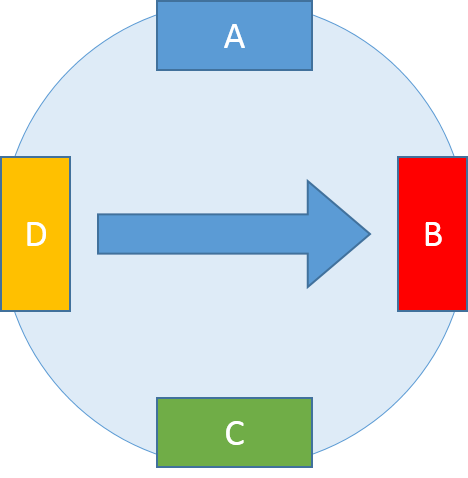
\includegraphics[width=0.9\linewidth]{step3}
		\end{figure}
	\end{minipage}
	\begin{minipage}[c]{0.24\textwidth}
		\begin{figure}
			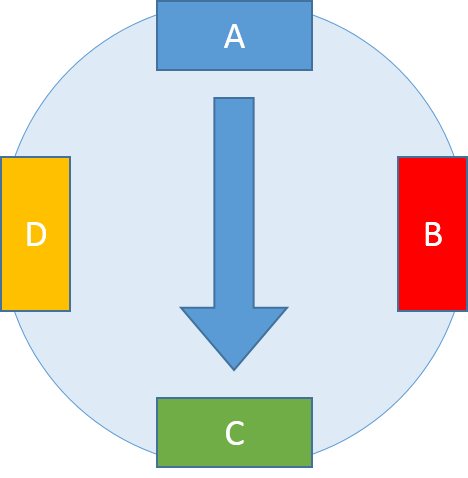
\includegraphics[width=0.9\linewidth]{step5}
		\end{figure}
	\end{minipage}
	\begin{minipage}[c]{0.24\textwidth}
		\begin{figure}
			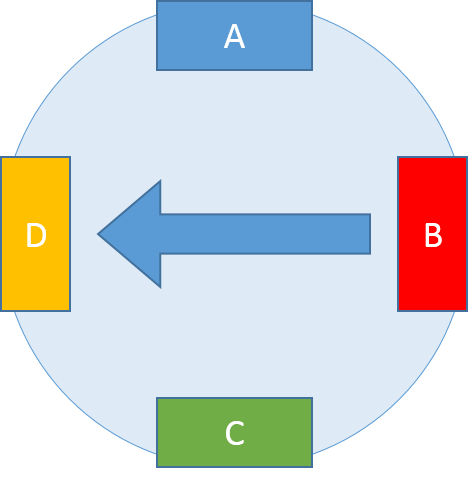
\includegraphics[width=0.9\linewidth]{step7}
		\end{figure}
	\end{minipage}
	\begin{center}
		Stepper Motor's positions in the wave stepping sequence
	\end{center}
\end{frame}

\subsection{Full Stepping}

\begin{frame}
	\frametitle{Full Stepping}
	\pause
	%Full stepping
	%It involves exciting two adjacent coils turn by turn in a circular fashion.
	\begin{table}
		\begin{tabular}{c c c c c}
			\toprule
			\textbf{Step} & \textbf{Coil A} & \textbf{Coil B} & \textbf{Coil C} & \textbf{Coil D}\\
			\midrule
			1 & 1 & 1 & 0 & 0 \\
			2 & 0 & 1 & 1 & 0 \\
			3 & 0 & 0 & 1 & 1 \\
			4 & 1 & 0 & 0 & 1 \\
			\bottomrule
		\end{tabular}
		\caption{Full stepping sequence}
	\end{table}
	%The table shows which coils are to be excited for generating the full stepping sequence. Notice that at each step exactly two coils are excited.
	%Now let's see what happens inside the motor when two coils are excited at once.
\end{frame}

\begin{frame}
	\frametitle{Full Stepping (contd.)}
	%As you can see, when two coils, say A and B are excited, the rotor settles between them. This results in a higher torque than that found in wave stepping.
	\begin{minipage}[c]{0.24\textwidth}
		\begin{figure}
			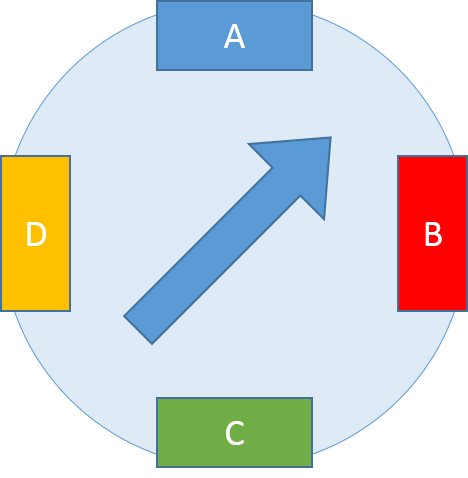
\includegraphics[width=0.9\linewidth]{step2}
		\end{figure}
	\end{minipage}
	\begin{minipage}[c]{0.24\textwidth}
		\begin{figure}
			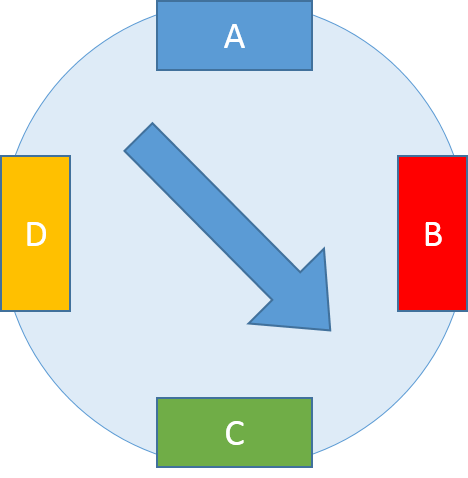
\includegraphics[width=0.9\linewidth]{step4}
		\end{figure}
	\end{minipage}
	\begin{minipage}[c]{0.24\textwidth}
		\begin{figure}
			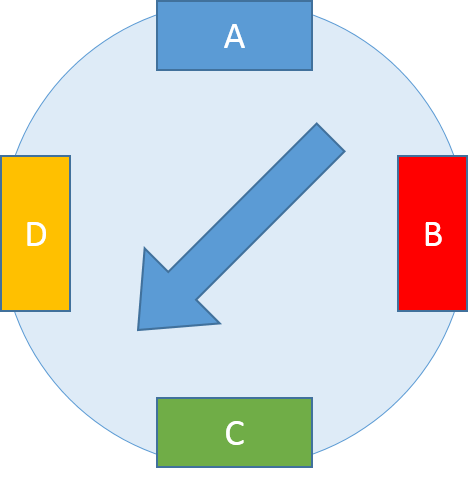
\includegraphics[width=0.9\linewidth]{step6}
		\end{figure}
	\end{minipage}
	\begin{minipage}[c]{0.24\textwidth}
		\begin{figure}
			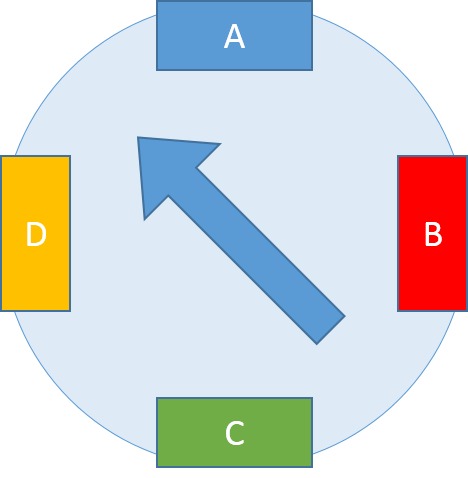
\includegraphics[width=0.9\linewidth]{step8}
		\end{figure}
	\end{minipage}
	\begin{center}
		Stepper Motor's positions in the full stepping sequence
	\end{center}
\end{frame}

\subsection{Half Stepping}

\begin{frame}
	\frametitle{Half Stepping}
	\pause
	%Half stepping
	%This stepping mode is a combination of wave and full stepping.
	\begin{table}
		\begin{tabular}{c c c c c}
			\toprule
			\textbf{Step} & \textbf{Coil A} & \textbf{Coil B} & \textbf{Coil C} & \textbf{Coil D}\\
			\midrule
			1 & 1 & 0 & 0 & 0 \\
			2 & 1 & 1 & 0 & 0 \\
			3 & 0 & 1 & 0 & 0 \\
			4 & 0 & 1 & 1 & 0 \\
			5 & 0 & 0 & 1 & 0 \\
			6 & 0 & 0 & 1 & 1 \\
			7 & 0 & 0 & 0 & 1 \\
			8 & 1 & 0 & 0 & 1 \\
			\bottomrule
		\end{tabular}
		\caption{Half stepping sequence}
	\end{table}
	%If you look closely, half stepping uses full stepping between the step positions of wave stepping. Let's see what happens inside the motor during this sequence.
\end{frame}

\begin{frame}
	\frametitle{Half Stepping (contd.)}
	%As you can see, there are 8 positions corresponding to the 8 steps shown in the previous table. It is called half stepping because it effectively halves the step angle and offers more resolution.
	\begin{minipage}[c]{0.24\textwidth}
		\begin{figure}
			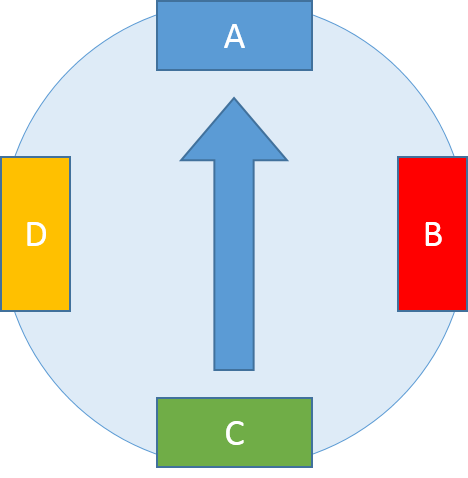
\includegraphics[width=0.9\linewidth]{step1}
		\end{figure}
	\end{minipage}
	\begin{minipage}[c]{0.24\textwidth}
		\begin{figure}
			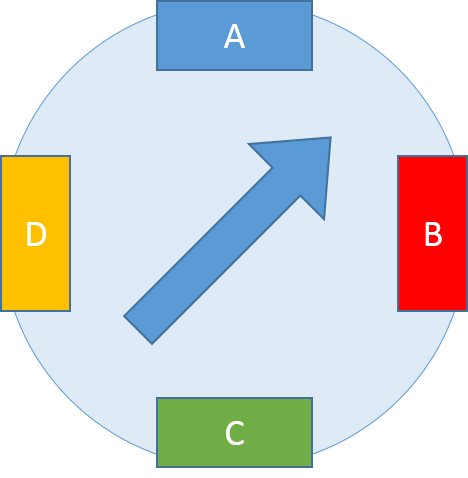
\includegraphics[width=0.9\linewidth]{step2}
		\end{figure}
	\end{minipage}
	\begin{minipage}[c]{0.24\textwidth}
		\begin{figure}
			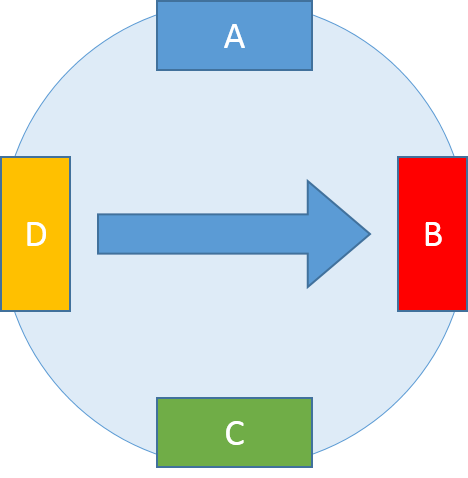
\includegraphics[width=0.9\linewidth]{step3}
		\end{figure}
	\end{minipage}
	\begin{minipage}[c]{0.24\textwidth}
		\begin{figure}
			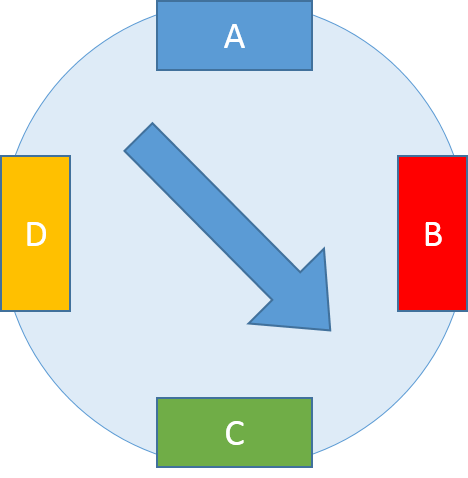
\includegraphics[width=0.9\linewidth]{step4}
		\end{figure}
	\end{minipage}
	\begin{minipage}[c]{0.24\textwidth}
		\begin{figure}
			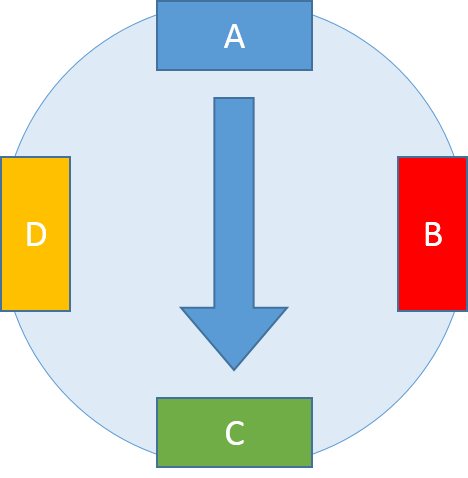
\includegraphics[width=0.9\linewidth]{step5}
		\end{figure}
	\end{minipage}
	\begin{minipage}[c]{0.24\textwidth}
		\begin{figure}
			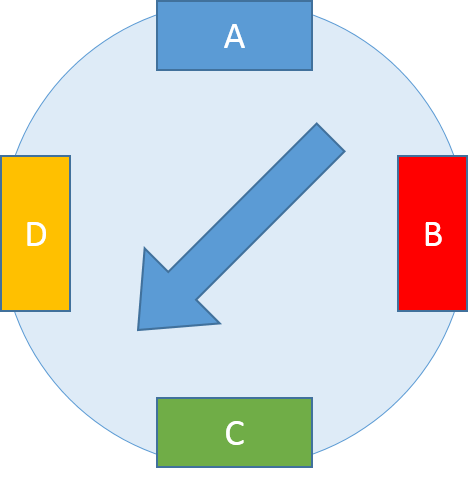
\includegraphics[width=0.9\linewidth]{step6}
		\end{figure}
	\end{minipage}
	\begin{minipage}[c]{0.24\textwidth}
		\begin{figure}
			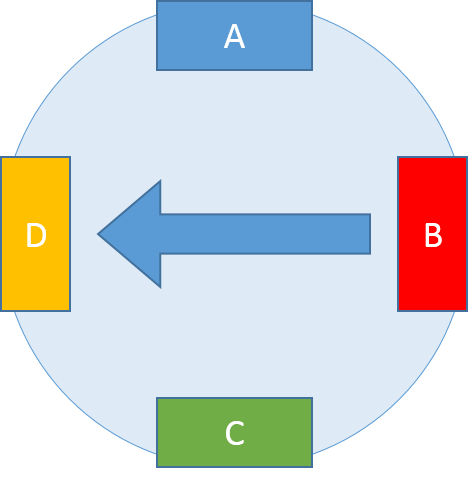
\includegraphics[width=0.9\linewidth]{step7}
		\end{figure}
	\end{minipage}
	\begin{minipage}[c]{0.24\textwidth}
		\begin{figure}
			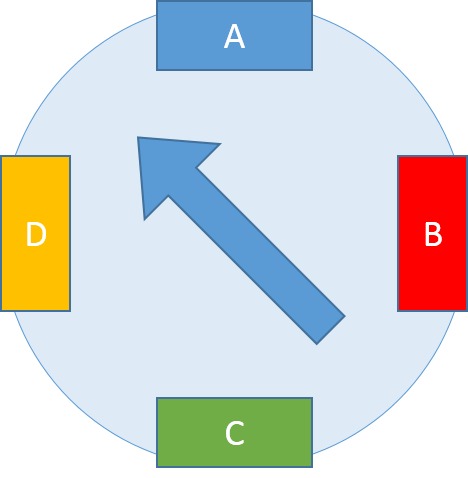
\includegraphics[width=0.9\linewidth]{step8}
		\end{figure}
	\end{minipage}
	
	\begin{center}
		Stepper Motor's positions in the half stepping sequence
	\end{center}

\end{frame}

\subsection{Comparison of stepping modes}

\begin{frame}
	\frametitle{Comparison of stepping modes}
	\pause
	%We will now see the differences and similarities between the 3 different stepping modes
	\begin{columns}[t]
		\column{.24\textwidth}
		\textbf{Stepping Mode}
		\begin{enumerate}
			\item Torque
			\item Vibration
			\item Speed
			\item Resolution
		\end{enumerate}
		
		
		\column{.24\textwidth}
		\textbf{Wave Stepping}
		\begin{enumerate}
			\item Lowest
			\item Intermediate
			\item Full
			\item Normal
		\end{enumerate}
		
		\column{.24\textwidth}
		\textbf{Full Stepping}
		\begin{enumerate}
			\item Highest
			\item Highest
			\item Full
			\item Normal
		\end{enumerate}
		
		\column{.24\textwidth}
		\textbf{Half Stepping}
		\begin{enumerate}
			\item Intermediate
			\item Lowest
			\item Halved
			\item Doubled
		\end{enumerate}
		
	\end{columns}
	%Talking about torque, since only one coil at a time is energised in wave stepping, its torque is the lowest. In full stepping, 2 coils are excited at once creating a larger attractive force resulting in a larger torque. Since half stepping excites 1 or 2 coils per step, the torque output is intermediate.
	
	%Vibration in a stepper motor increases with torque and decreases when the step angle decreases. Since wave stepping has low torque, but a step angle larger than half stepping, it has an intermediate level of vibration. Full stepping has higher torque resulting in more vibration and half stepping, due to a smaller step angle exhibits the least vibration.
	
	%Next is speed. Speed is equal to the step angle times the step frequency, since the step angle is the same for wave and full stepping, they have the same speed. For half stepping, the stepping angle is halved and thus the speed is also halved.
	
	%Resolution is fineness of control over rotational angle and is equal to the step angle. The step angle is equal for wave and full stepping while it is halved for half stepping.

\end{frame}

\section{Identifying the wires of a stepper motor}

\begin{frame}
	\begin{center}
		\textbf{\LARGE Identifying the wires of a stepper motor}
		%We will now learn how to identify the wires of a stepper motor.
	\end{center}
\end{frame}
%--------Video of practical identification of wires-----

\section{Stepper Motor Driver}

\begin{frame}
	\frametitle{Stepper Motor Driver Circuit}
	\begin{center}
		%This is the circuit diagram for the stepper motor driver
		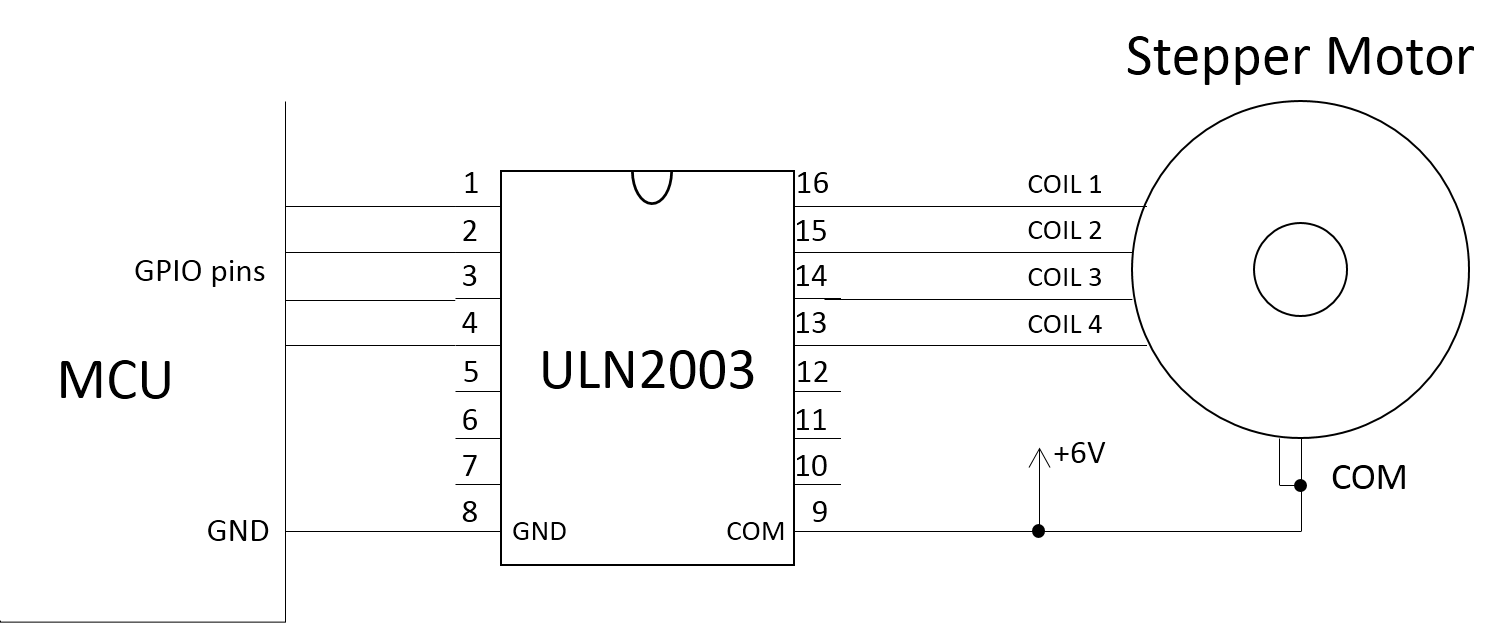
\includegraphics[width=\linewidth]{Driver}
		%The ULN2003 is a transistor array package of 7 transistors that are capable of switching 500 milli Amperes of current per transistor. The pins 1-7 are the inputs to the transistors, while the pins 16-10 are the corresponding open-collector outputs. All transistors have a commmon emitter that is connected to the ground at pin 8. The COM pin at pin 9 is connected externally to the supply voltage. The circuit is basically used to drive the stepper's high current windings by a microcontroller's General Purpose IO pins.
	\end{center}
\end{frame}

\section{Interfacing with LPC2148}

\subsection{GPIO pins}
\begin{frame}
	\frametitle{Interfacing with LPC2148}
	\framesubtitle{GPIO pins}
	%We will now discuss how to interface the ARM7 based Firebird V robot with the stepper motor using this circuit
	\pause
	\begin{center}
		\begin{table}
			\begin{tabular}{c c c}
			\toprule
			\textbf{JTAG connector pin} & \textbf{MCU pin} & \textbf{Connected to}\\
			\midrule
			11 & P1.26 & ULN2003 pin 1 \\
			13 & P1.27 & ULN2003 pin 2 \\
			5 & P1.28 & ULN2003 pin 3 \\
			9 & P1.29 & ULN2003 pin 4 \\
			4 & GND & ULN2003 pin 8 \\
			\bottomrule
			\end{tabular}
			\caption{GPIO pins used}
		\end{table}
		
		%These are the Firebird V robot's JTAG connector pins which we are going to use to connect to the driver circuit shown previously.
		%pin 11 on the JTAG connector i.e., P1.26 is connected to the ULN2003 driver IC's pin 1
		%pin 13 i.e., P1.27 is connected to the ULN2003 driver IC's pin 2
		%pin 5 i.e., P1.28 is connected to the ULN2003 driver IC's pin 3
		%pin 9 i.e., P1.29 is connected to the ULN2003 driver IC's pin 4
		%pin 4 i.e., Ground is connected to the ULN2003 driver IC's Ground on pin 8
		\pause
		\begin{figure}
			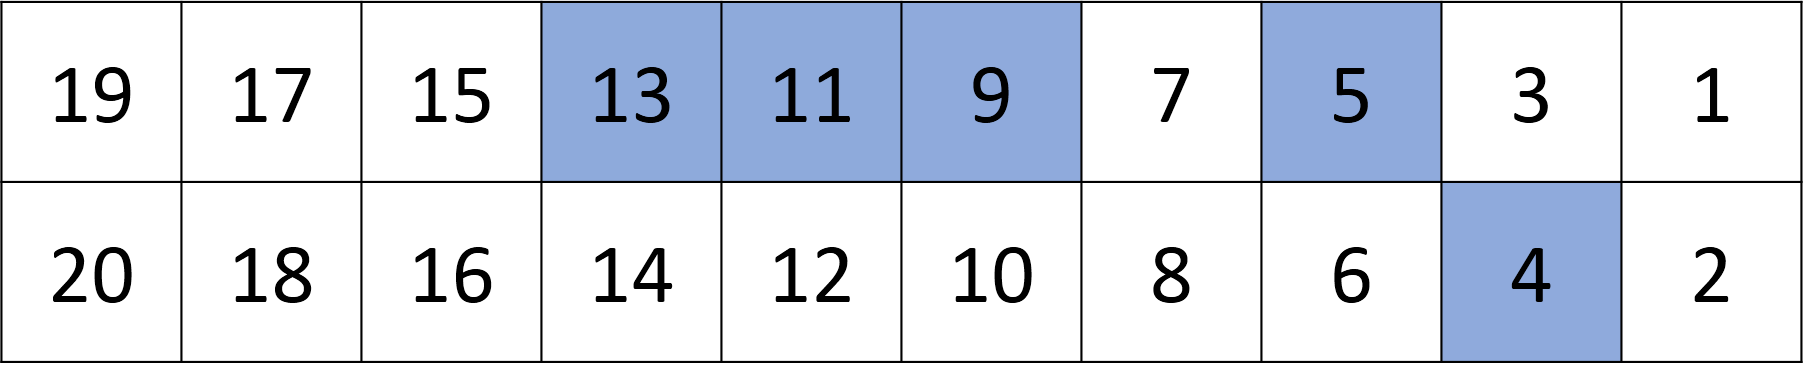
\includegraphics[width=0.5\linewidth]{pinnumbering}
			\caption{Pin numbering on the JTAG connector}
		\end{figure}
		%The pins are numbered on the connector as shown in the figure. We will be using the pins 11, 13, 5, 9 and 4. The numbering is done assuming you are looking into the 20-pin male FRC connector on the Firebird.
	\end{center}
\end{frame}


\subsection{Code}

\begin{frame}[shrink = 2,fragile]
	\frametitle{Interfacing with LPC2148}
	\framesubtitle{Code}
	%Now for an example, we will be rotating the stepper motor in one direction at a fixed speed for a complete revolution and then change its direction and repeat the process in the opposite direction. For this, we can either use delays between steps or we can use one of the timers for the delays. For this video we will be using simple delays for the job.
	
	\pause
	\begin{block}<1->{\#include}
		\begin{semiverbatim}
			\scriptsize{
\#include <lpc214x.h>
\#include "stepper.h"
			}
		\end{semiverbatim}
	\end{block}
	\pause
	%This is a list of headers to be included, which are: lpc214x.h and a custom header called stepper.h that contains the functions for controlling the GPIO pins of the stepper in different step modes.
	\begin{block}<1->{Main Program}
		\begin{semiverbatim}
			\scriptsize{
int direction = 1;
int count = 0;
int main(void)
\{
    stepper\_port\_init();\color{comment}//Initialize ports\color{black} \pause
    while(1)
    \{
        full\_step(direction); \pause
        DelaymSec(10); \color{comment}//10 ms between steps equals 100Hz\color{black} \pause
        if(count++ >= 200) \color{comment}//Change direction every revolution\color{black}
        \{
            direction = -1 * direction;
            count = 0;
        \}
    \}
\}
			}
		\end{semiverbatim}
	\end{block}
	%1:
	%Moving on to the main function, first we initialize the IO ports for the stepper motor.
	%2:
	%Then in an infinite while loop, we have a call to the function full(underscore)step which takes direction as argument and is defined in stepper.h and will be discussed in the next slide.
	%3:
	%This is followed by a delay of 10 milliseconds so that the resulting step frequency is 100Hz.
	%4:
	%direction here is a global variable that is initially set to +1 and is changed to -1 after every 200 steps by the following code which increments count in each iteration and changes direction from +1 to -1 and vice versa if count exceeds 200. It then resets the count to 0.
	%The stepper motor we use, completes a revolution in 200 steps. Modify this value if your stepper motor's steps per revolution value is different.
\end{frame}

\begin{frame}[shrink = 2,fragile]
	\frametitle{Interfacing with LPC2148}
	\framesubtitle{Code (contd.)}

%Now let's have a look at the port intialisation function, stepper(underscore)port(underscore)init. The function starts by setting the PINSEL2 register's bit 3 on and bits 2, 1 and 0 off. Bits 1 and 0 are reserved bits and bit 2 is set to zero to disable the JTAG functionality of the pins to allow us to use them as GPIO pins. The second line sets the four pins as output pins as specified in the #define constants COILAPIN, COILBPIN, COILCPIN and COILDPIN in the register represented by the constant STEPPERPORTDIR which equals IO1DIR, i.e., the port direction register for IO Port1.
%Using #define constants for ports and pins allow greater flexibility and reusability of code should you later decide to use another port or pin. Although it is used only once here, it will be used more often in the step functions that we will discuss later.
	\begin{block}<1->{Port Initialisation}
		\begin{semiverbatim}
			\scriptsize{
\#define STEPPERPORTDIR IO1DIR
\#define COILAPIN 26
\#define COILBPIN 27
\#define COILCPIN 28
\#define COILDPIN 29
void stepper\_port\_init()
\{
    PINSEL2 = (PINSEL2 \& 0x8);
    STEPPERPORTDIR |= (1<<COILAPIN) | (1<<COILBPIN) |
        (1<<COILCPIN) | (1<<COILDPIN);
\}
			}
		\end{semiverbatim}
	\end{block}
\end{frame}

%----------Show code in Keil uV4 IDE------------
%----------Show working video of the code-------
%So by now we have successfully understood the control of stepper motors and how to interface a stepper motor with the LPC2148 based Firebird V robotics platform. You may modify the code to experiment with different stepping modes or by setting it to specific angles or by using timers or basically anything that your imagination leads you to.

\begin{frame}
	\begin{center}
		\textbf{\LARGE Thank You!} \\
		\vspace{20pt}
		\scriptsize Send your queries to: 
		\href{mailto:helpdesk@e-yantra.org} {\color{blue}helpdesk@e-yantra.org \color{black}}
	\end{center}
	%With this we have reached the end of this video tutorial. Thank you for listening! For any doubts or suggestions feel free to mail them at helpdesk@e(hyphen)yantra(dot)org
	%This is Joel Pinto signing off!
\end{frame}

\end{document}